\subsection{Recovery in Winding Counterflow Tasks}
\label{sec:winding}
Three full-height walls with alternating openings produce repeated turns and opposing traffic. The representative task contains five UAVs, 2.2 m openings, and a fixed 24 s flight horizon with $h=0.2$ s. The spatial and relative growth limits, motion envelope, footprint, acceptance thresholds, and 30 s planning budget remain unchanged. A common 0.325 m static-guide grid resolves the openings. Each method receives the same saved reference and is charged the same measured initialization time. Hard RSC--iterative retains its reconstruction loop.

An exploratory search identified the task in Figure~\ref{fig:winding-recovery}. In the three initial paired executions of this task, proposed LIOM accepted the motion after five recovery rounds in 26.59--27.18 s. Soft LIOM also accepted all three executions, taking 25.33--25.72 s. Hard RSC--iterative completed eight reconstruction rounds per execution without acceptance within the budget. These repetitions characterize one physical task. Section~\ref{sec:external} reports a further paired execution alongside the nonlinear and sequential-convex methods. The accepted motion has minimum center separation 1.086 m, minimum obstacle surface clearance 0.495 m, maximum speed 3.577 m/s, and maximum acceleration 2.990 m/s$^2$; the respective requirements are 0.60 m, 0.10 m, 4 m/s, and 3 m/s$^2$.

An independent phase-I linear program minimizes a common row-scaled violation of the initial hard-RSC constraints. Its primal and dual objectives both equal 0.21915, with primal residual below $5\times10^{-14}$ and dual stationarity residual below $2\times10^{-17}$. Removing the relative rows alone, or the kinematic equalities alone, gives zero phase-I objective. These diagnostic checks identify an incompatibility between the selected relative restrictions and exact motion consistency. The complete returned motion satisfies both requirements after reconstruction. The diagnostic relaxations are used only to identify the conflict.

\begin{figure}[htbp]
\begin{adjustwidth}{-\extralength}{0cm}\centering
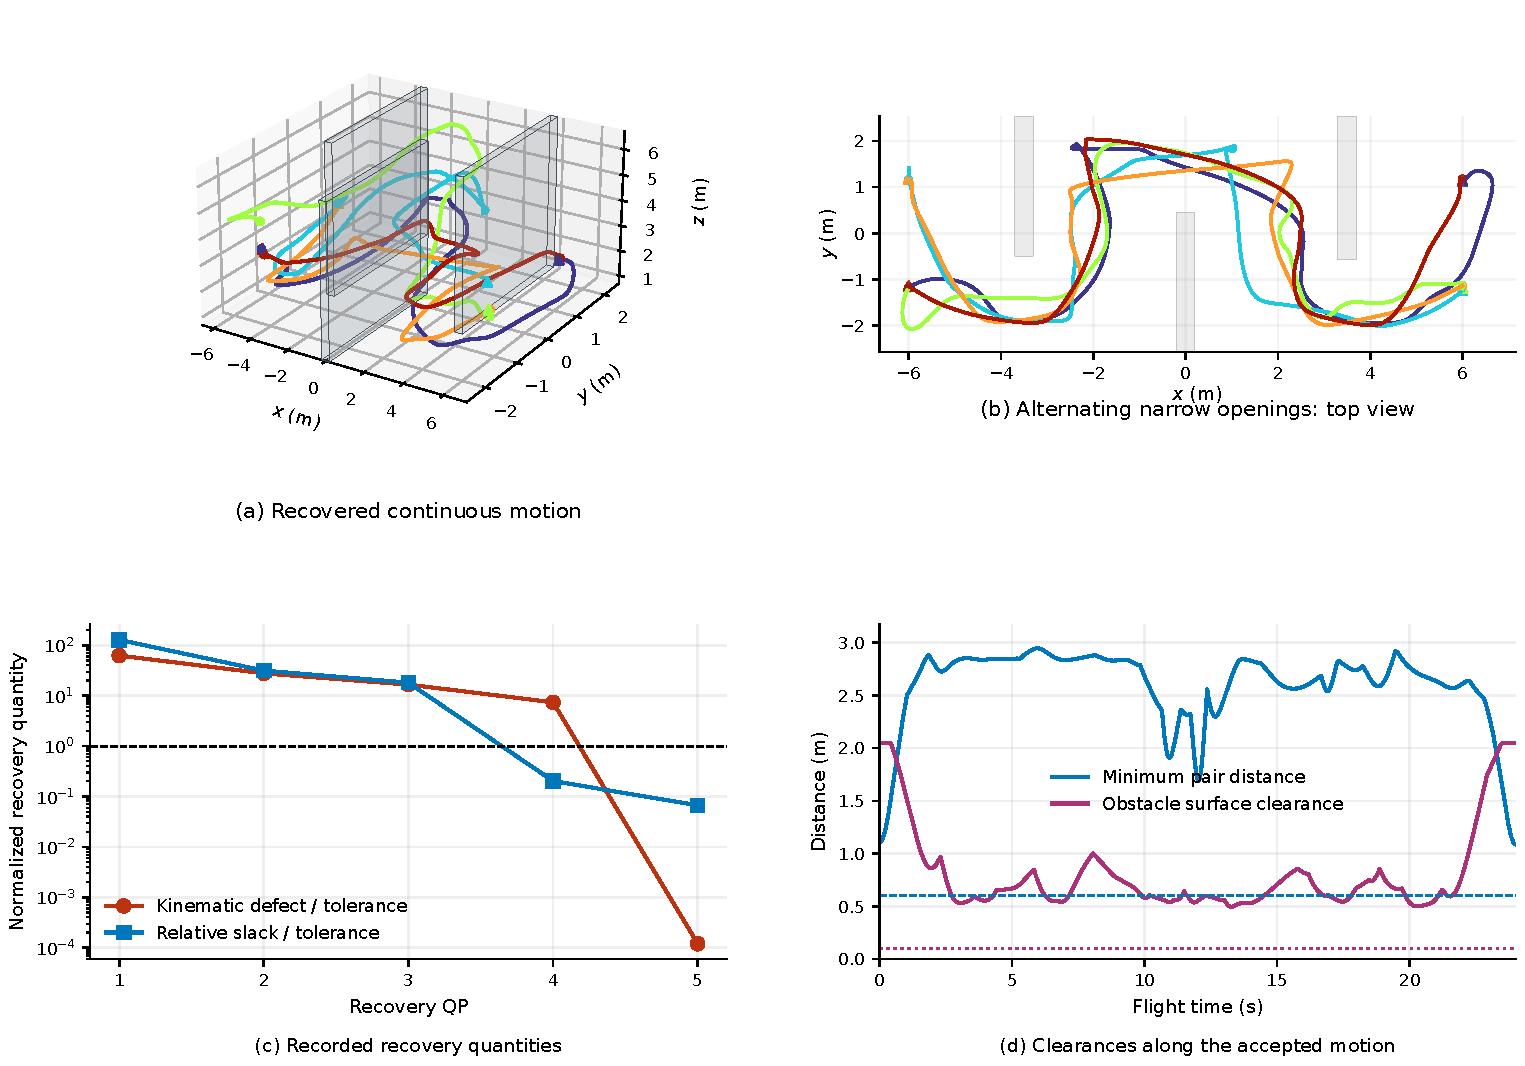
\includegraphics[width=\fulllength]{figures_revision/winding_recovery_case.pdf}
\caption{Recovery in a winding counterflow task. Colors identify UAVs. The recovery quantities are divided by their acceptance thresholds; the dashed unit line marks numerical recovery. The clearance curves visualize the integrated motion, whose acceptance is determined by complete-interval checks.\label{fig:winding-recovery}}
\end{adjustwidth}\end{figure}

A separate set of 12 previously untested random layouts contains a second recovered task whose initial hard QP has matching phase-I primal and dual objectives of 0.35420. The proposed method returns a checked motion for this task, while iterative hard RSC exhausts the common budget. This independently generated case supports the same conflict mechanism. The complete 12-layout outcomes and all exploratory records accompany the data.

Figure~\ref{fig:winding-map} varies physical opening width, team size, and prescribed flight time around the identified geometry. The nominal corridor-growth limits are unchanged. Both methods accept the three-UAV tasks. With five UAVs and 2.2 m openings, proposed LIOM additionally accepts the 24 s and 28 s tasks. Widening the openings permits both methods to succeed. The map locates the additional recovery region under physical congestion; it also shows where neither method returns an accepted motion within the common budget.
\begin{figure}[htbp]
\begin{adjustwidth}{-\extralength}{0cm}\centering
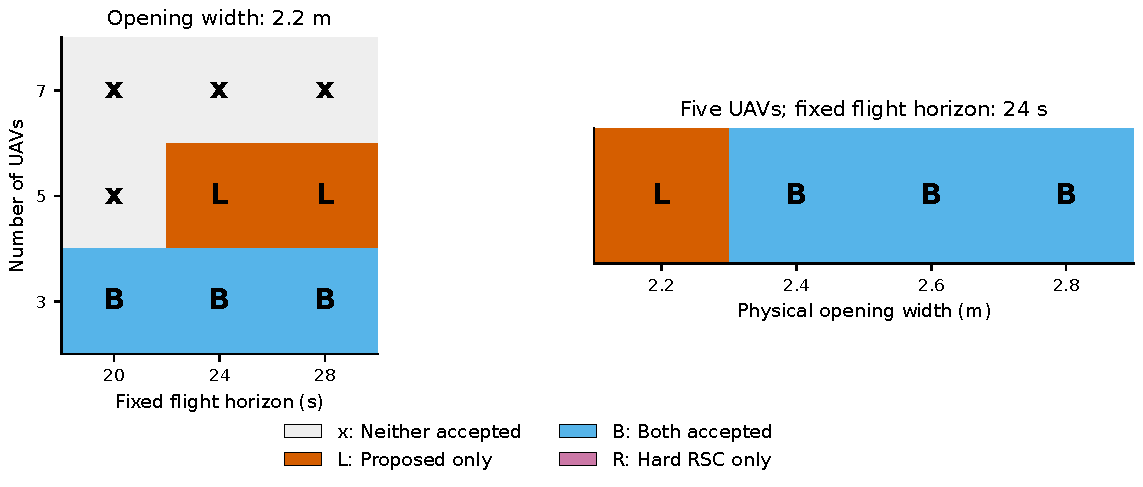
\includegraphics[width=\fulllength]{figures_revision/physical_recovery_map.pdf}
\caption{Exploratory physical-parameter map around the same winding layout. Letters supplement color: B, both accepted; L, proposed LIOM only; R, Hard RSC--iterative only; x, neither accepted. Twelve distinct settings are evaluated; the five-UAV, 24 s, 2.2 m setting appears in both panels. Every setting uses the same reference for both methods and the same 30 s budget.\label{fig:winding-map}}
\end{adjustwidth}\end{figure}
